\documentclass[12pt, titlepage]{article}


\usepackage{fullpage}
\usepackage[round]{natbib}
\usepackage{multirow}
\usepackage{booktabs}
\usepackage{tabularx}
\usepackage{graphicx}
\usepackage{float}
\usepackage{hyperref}
\hypersetup{
    colorlinks,
    citecolor=blue,
    filecolor=black,
    linkcolor=red,
    urlcolor=blue
}

%% Comments

\usepackage{color}

\newif\ifcomments\commentstrue %displays comments
%\newif\ifcomments\commentsfalse %so that comments do not display

\ifcomments
\newcommand{\authornote}[3]{\textcolor{#1}{[#3 ---#2]}}
\newcommand{\todo}[1]{\textcolor{red}{[TODO: #1]}}
\else
\newcommand{\authornote}[3]{}
\newcommand{\todo}[1]{}
\fi

\newcommand{\wss}[1]{\authornote{blue}{SS}{#1}} 
\newcommand{\plt}[1]{\authornote{magenta}{TPLT}{#1}} %For explanation of the template
\newcommand{\an}[1]{\authornote{cyan}{Author}{#1}}

%% Common Parts

\newcommand{\progname}{2D-RAPP} % PUT YOUR PROGRAM NAME HERE
\newcommand{\authname}{Ziyang(Ryan) Fang} % AUTHOR NAMES                  

\usepackage{hyperref}
    \hypersetup{colorlinks=true, linkcolor=blue, citecolor=blue, filecolor=blue,
                urlcolor=blue, unicode=false}
    \urlstyle{same}
                                


\newcounter{acnum}
\newcommand{\actheacnum}{AC\theacnum}
\newcommand{\acref}[1]{AC\ref{#1}}

\newcounter{ucnum}
\newcommand{\uctheucnum}{UC\theucnum}
\newcommand{\uref}[1]{UC\ref{#1}}

\newcounter{mnum}
\newcommand{\mthemnum}{M\themnum}
\newcommand{\mref}[1]{M\ref{#1}}

\begin{document}

\title{Module Guide for \progname{}} 
\author{\authname}
\date{\today}

\maketitle

\pagenumbering{roman}

\section{Revision History}

\begin{tabularx}{\textwidth}{p{3cm}p{2cm}X}
\toprule {\bf Date} & {\bf Version} & {\bf Notes}\\
\midrule
March 19 2025 & 1.0 & Notes\\
April 05 2025 & 2.0 & Notes\\
\bottomrule
\end{tabularx}

\newpage

\section{Reference Material}

This section records information for easy reference.

\subsection{Abbreviations and Acronyms}

\renewcommand{\arraystretch}{1.2}
\begin{tabular}{l l} 
  \toprule		
  \textbf{symbol} & \textbf{description}\\
  \midrule 
  A & Assumption\\
  DD & Data Definition\\
  GD & General Definition\\
  GS & Goal Statement\\
  IM & Instance Model\\
  LC & Likely Change\\
  PS & Physical System Description\\
  R & Requirement\\
  SRS & Software Requirements Specification\\
  TM & Theoretical Model\\
  IK & Inverse Kinematics \\
  FK & Forward Kinematics \\
  A* & A-star Pathfinding Algorithm \\
  DOF & Degrees of Freedom \\
  EE & End-Effector \\
  % \progname{} & 2DPL\\
  2D-RAPP & 2D Robot Arm Path Planning\\
  \bottomrule
\end{tabular}\\

\newpage

\tableofcontents

\listoftables

\listoffigures

\newpage

\pagenumbering{arabic}

\section{Introduction}

Decomposing a system into modules is a commonly accepted approach to developing
software.  A module is a work assignment for a programmer or programming
team~\citep{ParnasEtAl1984}.  We advocate a decomposition
based on the principle of information hiding~\citep{Parnas1972a}.  This
principle supports design for change, because the ``secrets'' that each module
hides represent likely future changes.  Design for change is valuable in SC,
where modifications are frequent, especially during initial development as the
solution space is explored.  

Our design follows the rules layed out by \citet{ParnasEtAl1984}, as follows:
\begin{itemize}
\item System details that are likely to change independently should be the
  secrets of separate modules.
\item Each data structure is implemented in only one module.
\item Any other program that requires information stored in a module's data
  structures must obtain it by calling access programs belonging to that module.
\end{itemize}

After completing the first stage of the design, the SRS, the MG is developed~\citep{ParnasEtAl1984}. The MG
specifies the modular structure of the system and is intended to allow both
designers and maintainers to easily identify the parts of the software.  The
potential readers of this document are as follows:

\begin{itemize}
\item New project members: This document can be a guide for a new project member
  to easily understand the overall structure and quickly find the
  relevant modules they are searching for.
\item Maintainers: The hierarchical structure of the module guide improves the
  maintainers' understanding when they need to make changes to the system. It is
  important for a maintainer to update the relevant sections of the document
  after changes have been made.
\item Designers: Once the module guide has been written, it can be used to
  check for consistency, feasibility, and flexibility. Designers can verify the
  system in various ways, such as consistency among modules, feasibility of the
  decomposition, and flexibility of the design.
\end{itemize}

The rest of the document is organized as follows. Section
\ref{SecChange} lists the anticipated and unlikely changes of the software
requirements. Section \ref{SecMH} summarizes the module decomposition that
was constructed according to the likely changes. Section \ref{SecConnection}
specifies the connections between the software requirements and the
modules. Section \ref{SecMD} gives a detailed description of the
modules. Section \ref{SecTM} includes two traceability matrices. One checks
the completeness of the design against the requirements provided in the SRS. The
other shows the relation between anticipated changes and the modules. Section
\ref{SecUse} describes the use relation between modules.

\section{Anticipated and Unlikely Changes} \label{SecChange}

This section lists possible changes to the system. According to the likeliness
of the change, the possible changes are classified into two
categories. Anticipated changes are listed in Section \ref{SecAchange}, and
unlikely changes are listed in Section \ref{SecUchange}.

\subsection{Anticipated Changes} \label{SecAchange}

Anticipated changes are the source of the information that is to be hidden
inside the modules. Ideally, changing one of the anticipated changes will only
require changing the one module that hides the associated decision. The approach
adapted here is called design for
change.

\begin{description}
\item[\refstepcounter{acnum} \actheacnum \label{ac1}:] The specific
  hardware on which the software is running.
\item[\refstepcounter{acnum} \actheacnum \label{ac2}:] The format of the initial input data may change, while still assuming a 2D environment.
\item[\refstepcounter{acnum} \actheacnum \label{ac3}:] The format of the initial input parameters may change, but the fundamental 2D assumption remains.
\item[\refstepcounter{acnum} \actheacnum \label{ac4}:]The constraints on the input parameters

\item[\refstepcounter{acnum} \actheacnum \label{ac5}:] The format of the final output data.

\item[\refstepcounter{acnum} \actheacnum \label{ac6}:] The constraints on the output results.
\item[\refstepcounter{acnum} \actheacnum \label{ac7}:] How the geometric constraints for obstacle avoidance are defined using input obstacle parameters.
\item[\refstepcounter{acnum} \actheacnum \label{ac8}:] How distance-based inverse kinematic equations are formulated based on input robot parameters
\item[\refstepcounter{acnum} \actheacnum \label{ac9}:] How the overall control flow of the path-planning calculations and iterations is orchestrated.
\item[\refstepcounter{acnum} \actheacnum \label{ac10}:] The implementation used for storing and managing the joint-space grid or graph data structure.
\item[\refstepcounter{acnum} \actheacnum \label{ac11}:] The algorithm selected for solving the inverse kinematics (IK) optimization problem.
\item[\refstepcounter{acnum} \actheacnum \label{ac12}:] The method or library used for visualizing and plotting robot paths and configurations.
\end{description}

\subsection{Unlikely Changes} \label{SecUchange}

The module design should be as general as possible. However, a general system is
more complex. Sometimes this complexity is not necessary. Fixing some design
decisions at the system architecture stage can simplify the software design. If
these decision should later need to be changed, then many parts of the design
will potentially need to be modified. Hence, it is not intended that these
decisions will be changed.

\begin{description}
  \item[\refstepcounter{ucnum} \uctheucnum \label{uc1}:] The fundamental requirement of navigating from a start position to a goal position remains unchanged.
  \item[\refstepcounter{ucnum} \uctheucnum \label{uc2}:] The system assumes a two-dimensional environment, which is not expected to change.
  \item[\refstepcounter{ucnum} \uctheucnum \label{uc3}:] The fundamental requirement of determining a feasible path from a single start position to a single goal position remains unchanged.
  \item[\refstepcounter{ucnum} \uctheucnum \label{uc4}:] The system assumes a strictly two-dimensional planar environment.

  \item[\refstepcounter{ucnum} \uctheucnum \label{uc5}:] The robot arm is assumed to have a serial manipulator structure, which will remain constant.

  \item[\refstepcounter{ucnum} \uctheucnum \label{uc6}:] Obstacles within the environment are static and their positions and sizes do not change during path planning.

  \item[\refstepcounter{ucnum} \uctheucnum \label{uc7}:] The robot will always have exactly one start and one goal configuration per planning task; handling multiple simultaneous goal points is out of scope.
\end{description}

\section{Module Hierarchy} \label{SecMH}

This section provides an overview of the module design. Modules are summarized
in a hierarchy decomposed by secrets in Table \ref{TblMH}. The modules listed
below, which are leaves in the hierarchy tree, are the modules that will
actually be implemented.

\begin{description}
\item [\refstepcounter{mnum} \mthemnum \label{mHH1}:] Hardware-Hiding Module
\item [\refstepcounter{mnum} \mthemnum \label{mHH2}:] Input Parameters Module
\item [\refstepcounter{mnum} \mthemnum \label{mHH3}:] Output Format Module
\item [\refstepcounter{mnum} \mthemnum \label{mHH4}:] Output Verification Module
\item [\refstepcounter{mnum} \mthemnum \label{mHH5}:] Path Planning Module
\item [\refstepcounter{mnum} \mthemnum \label{mHH6}:] Collision Detection Module
\item [\refstepcounter{mnum} \mthemnum \label{mHH7}:] Inverse Kinematics Solver Module
\item [\refstepcounter{mnum} \mthemnum \label{mHH8}:] Plotting Module
\item [\refstepcounter{mnum} \mthemnum \label{mHH9}:] Configuration Management Module
\item [\refstepcounter{mnum} \mthemnum \label{mHH10}:] Logging and Debugging Module
\item [\refstepcounter{mnum} \mthemnum \label{mHH11}:] Control Module
\item [\refstepcounter{mnum} \mthemnum \label{mHH12}:] Data Tpyes Module
\end{description}


\begin{table}[h!]
  \centering
  \begin{tabular}{p{0.3\textwidth} p{0.6\textwidth}}
  \toprule
  \textbf{Level 1} & \textbf{Level 2}\\
  \midrule
  \textbf{Hardware Hiding} & \\ 
  \midrule
  \multirow{6}{0.3\textwidth}{\textbf{Behaviour Hiding}} 
  & Input Parameters Module \\ 
  & Output Format Module \\ 
  & Output Verification Module \\ 
  & Inverse Kinematics Solver Module \\ 
  & Configuration Management Module \\ 
  & Path Planning Module \\ 
  & Collision Detection Module \\ 
  & Controll Module\\
  & Data Types Module\\
  \midrule
  \multirow{1}{0.3\textwidth}{\textbf{Software Decision}} 
  & Plotting Module \\ 
  \bottomrule
  \end{tabular}
  \caption{Module Hierarchy}
  \label{TblMH}
\end{table}
  

\section{Connection Between Requirements and Design} \label{SecConnection}

The design of the system is intended to satisfy the requirements developed in
the SRS. In this stage, the system is decomposed into modules. The connection
between requirements and modules is listed in Table~\ref{TblRT}.

% \begin{table}[h] \centering \begin{tabular}{p{0.55\textwidth} p{0.35\textwidth}} \toprule \textbf{Requirement} & \textbf{Implemented by Module} \\
%    \midrule
%  System must accept and process user-defined parameters such as robot dimensions, joint lengths, and obstacle positions. & Input Parameters Module, Configuration Management Module \\

%   System must represent obstacles and detect potential collisions between the robot and obstacles. & Collision Detection Module \\
  
%   System must compute a feasible collision-free path from the initial to goal configuration. & Path Planning Module \\
  
%   System must determine accurate joint positions and angles based on distance-geometric methods. & Inverse Kinematics Solver Module \\
  
%   System must output calculated paths clearly for validation and analysis. & Output Format Module, Plotting Module \\
  
%   System must verify the feasibility and correctness of output results. & Output Verification Module \\
  
%   System must provide logging capabilities for monitoring system execution and debugging purposes. & Logging and Debugging Module \\
%   \bottomrule \end{tabular} \caption{ Requirement-Module Traceability Matrix} 
%   \label{Tb2RT}
%  \end{table}


\section{Module Decomposition} \label{SecMD}

Modules are decomposed according to the principle of ``information hiding''
proposed by \citet{ParnasEtAl1984}. The \emph{Secrets} field in a module
decomposition is a brief statement of the design decision hidden by the
module. The \emph{Services} field specifies \emph{what} the module will do
without documenting \emph{how} to do it. For each module, a suggestion for the
implementing software is given under the \emph{Implemented By} title. If the
entry is \emph{OS}, this means that the module is provided by the operating
system or by standard programming language libraries.  \emph{\progname{}} means the
module will be implemented by the \progname{} software.

Only the leaf modules in the hierarchy have to be implemented. If a dash
(\emph{--}) is shown, this means that the module is not a leaf and will not have
to be implemented.

\subsection{Hardware Hiding Modules (\mref{mHH1})}

\begin{description}
\item[Secrets:]The data structure and algorithm used to implement the virtual
  hardware.
\item[Services:]Serves as a virtual hardware used by the rest of the
  system. This module provides the interface between the hardware and the
  software. So, the system can use it to display outputs or to accept inputs.
\item[Implemented By:] OS
\end{description}

\subsection{Behaviour-Hiding Module}

\begin{description}
\item[Secrets:]The contents of the required behaviours.
\item[Services:]Includes programs that provide externally visible behaviour of
  the system as specified in the software requirements specification (SRS)
  documents. This module serves as a communication layer between the
  hardware-hiding module and the software decision module. The programs in this
  module will need to change if there are changes in the SRS.
\item[Implemented By:] OS or Simulation Framework
\end{description}

\subsubsection{Input Parameters Module (\mref{mHH2})}

\begin{description}
\item[Secrets:] The structure, format, and validation rules of the robot parameters, obstacle data, and environment definitions.
\item[Services:] Accepts input parameters from the user, verifies the correctness and completeness of the input parameters, and converts them into appropriate internal data structures for further processing.
\item[Implemented By:] 2D Robot Arm Path Planner
\item[Type of Module:] Abstract Data Type
\end{description}

\subsubsection{Output Format Module (\mref{mHH3})}

\begin{description}
\item[Secrets:] The structure and format of the system's output data, including joint positions, angles, and planned paths.
\item[Services:] Provides formatted output data after path planning and inverse kinematics computations, enabling further visualization or verification.
\item[Implemented By:] 2D Robot Arm Path Planner
\item[Type of Module:] Abstract Data Type
\end{description}

\subsubsection{Output Verification Module (\mref{mHH4})}

\begin{description}
\item[Secrets:] The criteria and methods used to validate the computed paths and configurations.
\item[Services:] Verifies the correctness and feasibility of computed paths, ensuring there are no collisions and all constraints are satisfied. Generates warnings or errors when violations are detected.
\item[Implemented By:] 2D Robot Arm Path Planner
\item[Type of Module:] Abstract Object
\end{description}

\subsubsection{Path Planning Module (\mref{mHH5})}

\begin{description}
\item[Secrets:] The algorithm and logic used to plan collision-free paths from start to goal configuration.
\item[Services:] Calculates feasible paths using provided obstacle information, initial and goal configurations. Ensures obstacle avoidance through distance-geometric and graph-based methods.
\item[Implemented By:] 2D Robot Arm Path Planner
\item[Type of Module:] Abstract Object
\end{description}

\subsubsection{Collision Detection Module (\mref{mHH6})}

\begin{description}
\item[Secrets:] The algorithms and conditions for detecting collisions between the robot arm and environment obstacles.
\item[Services:] Determines if a specific robot configuration or path results in a collision. Reports detailed collision information to path planning and verification modules.
\item[Implemented By:] 2D Robot Arm Path Planner
\item[Type of Module:] Abstract Object
\end{description}

\subsubsection{Inverse Kinematics Solver Module (\mref{mHH7})}

\begin{description}
\item[Secrets:] The mathematical methods and algorithms used for solving the inverse kinematics problem based on distance-geometric representation.
\item[Services:] Computes robot joint angles and positions from a given path. Provides accurate geometric conversions for the planned trajectory.
\item[Implemented By:] 2D Robot Arm Path Planner
\item[Type of Module:] Abstract Data Type
\end{description}

\subsubsection{Configuration Management Module (\mref{mHH9})}

\begin{description}
\item[Secrets:] The management, storage, and retrieval methods for system configuration parameters such as robot dimensions, joint constraints, and obstacle definitions.
\item[Services:] Provides centralized management of configuration parameters, allows consistent and efficient access to these parameters by other modules.
\item[Implemented By:] 2D Robot Arm Path Planner
\item[Type of Module:] Abstract Data Type
\end{description}




\subsection{Software Decision Module}

\begin{description}
\item[Secrets:] The design decision based on mathematical theorems, physical facts, or programming considerations. The secrets of this module are \emph{not} described in the SRS.
\item[Services:] Includes data structures and algorithms used in the system that do not provide direct interaction with the user.
\item[Implemented By:] Python (using standard libraries and third-party packages)
\end{description}

\subsubsection{Plotting Module (\mref{mHH8})}

\begin{description}
\item[Secrets:] The choice of visualization libraries and plotting algorithms for displaying robot configurations and paths.
\item[Services:] Generates graphical visualizations of robot arm configurations, joint trajectories, and obstacle environments. Facilitates analysis and debugging by providing clear visual representations of results.
\item[Implemented By:] Matplotlib (Python)
\item[Type of Module:] Library
\end{description}

\subsubsection{Logging and Debugging Module (\mref{mHH10})}

\begin{description}
\item[Secrets:] The selection and configuration of logging libraries and debugging tools.
\item[Services:] Provides logging of system states, events, exceptions, and debugging information during execution. Enables easier tracing of errors and verification of software correctness and performance.
\item[Implemented By:] Python logging module
\item[Type of Module:] Library
\end{description}

\subsubsection{Control Module (\mref{mHH11})}

\begin{description} \item[Secrets:] The logic and sequencing of interactions among different modules, including the order of invocation for path planning, collision detection, inverse kinematics solving, and output verification.

\item[Services:] Coordinates and manages the workflow of the system by invoking appropriate modules in the correct order. Specifically, it obtains input parameters, triggers path planning (using A*), performs collision checks, computes inverse kinematics, verifies output correctness, and generates final results for plotting and logging.

\item[Implemented By:] 2D Robot Arm Path Planner

\item[Type of Module:] Abstract Object \end{description}

\subsubsection{Data Types Module (\mref{mHH12})}

\begin{description}
  \item[Secrets:] The internal representations and definitions of abstract data types (ADTs) such as \texttt{Config}, \texttt{Path}, \texttt{ObstacleT}, \texttt{Obstacles}, and \texttt{RobotParams}, including how joint limits, link lengths, and geometric primitives are encoded.

  \item[Services:] Provides shared type definitions for all modules. These include representations of robot joint configurations, obstacle shapes, kinematic parameters, and motion paths. All modules depend on these definitions for consistent data exchange and interface specification.

  \item[Implemented By:] 2D Robot Arm Path Planner

  \item[Type of Module:] Pure Template
\end{description}


\section{Traceability Matrix} \label{SecTM}

This section shows two traceability matrices: between the modules and the
requirements and between the modules and the anticipated changes.

% the table should use mref, the requirements should be named, use something
% like fref
\begin{table}[H]
  \centering
  \begin{tabular}{p{0.2\textwidth} p{0.6\textwidth}}
  \toprule
  \textbf{Requirement} & \textbf{Modules} \\
  \midrule
  R1 & \mref{mHH2}, \mref{mHH9}, \mref{mHH11}, \mref{mHH12} \\
  R2 & \mref{mHH2}, \mref{mHH3}, \mref{mHH11}, \mref{mHH12} \\
  R3 & \mref{mHH5}, \mref{mHH6}, \mref{mHH7}, \mref{mHH11}, \mref{mHH12} \\
  R4 & \mref{mHH4}, \mref{mHH6}, \mref{mHH7}, \mref{mHH11}, \mref{mHH12} \\
  R5 & \mref{mHH3}, \mref{mHH8}, \mref{mHH10},\mref{mHH11}, \mref{mHH12} \\
  \bottomrule
  \end{tabular}
  \caption{Trace Between Requirements and Modules}
  \label{TblRT}
  \end{table}
  

\begin{table}[H]
  \centering
  \begin{tabular}{p{0.2\textwidth} p{0.6\textwidth}}
  \toprule
  \textbf{AC} & \textbf{Modules}\\
  \midrule
  \acref{ac1} & \mref{mHH1}\\
  \acref{ac2} & \mref{mHH2} , \mref{mHH12}\\
  \acref{ac3} & \mref{mHH2}, \mref{mHH9}, \mref{mHH12}\\
  \acref{ac4} & \mref{mHH2}, \mref{mHH9}, \mref{mHH12}\\
  \acref{ac5} & \mref{mHH3}, \mref{mHH12}\\
  \acref{ac6} & \mref{mHH4}, \mref{mHH12}\\
  \acref{ac7} & \mref{mHH6}, \mref{mHH5}, \mref{mHH12}\\
  \acref{ac8} & \mref{mHH7}, \mref{mHH12}\\
  \acref{ac9} & \mref{mHH5}, \mref{mHH10}, \mref{mHH11}\\
  \acref{ac10} & \mref{mHH5}, \mref{mHH11}, \mref{mHH12}\\
  \acref{ac11} & \mref{mHH7}, \mref{mHH11}\\
  \acref{ac12} & \mref{mHH8}\\
  \bottomrule
  \end{tabular}
  \caption{Trace Between Anticipated Changes and Modules}
  \label{TblACT}
  \end{table}
  

\section{Use Hierarchy Between Modules} \label{SecUse}

In this section, the uses hierarchy between modules is
provided. \citet{Parnas1978} said of two programs A and B that A {\em uses} B if
correct execution of B may be necessary for A to complete the task described in
its specification. That is, A {\em uses} B if there exist situations in which
the correct functioning of A depends upon the availability of a correct
implementation of B.  Figure \ref{FigUH} illustrates the use relation between
the modules. It can be seen that the graph is a directed acyclic graph
(DAG). Each level of the hierarchy offers a testable and usable subset of the
system, and modules in the higher level of the hierarchy are essentially simpler
because they use modules from the lower levels.


\begin{figure}[H]
\centering
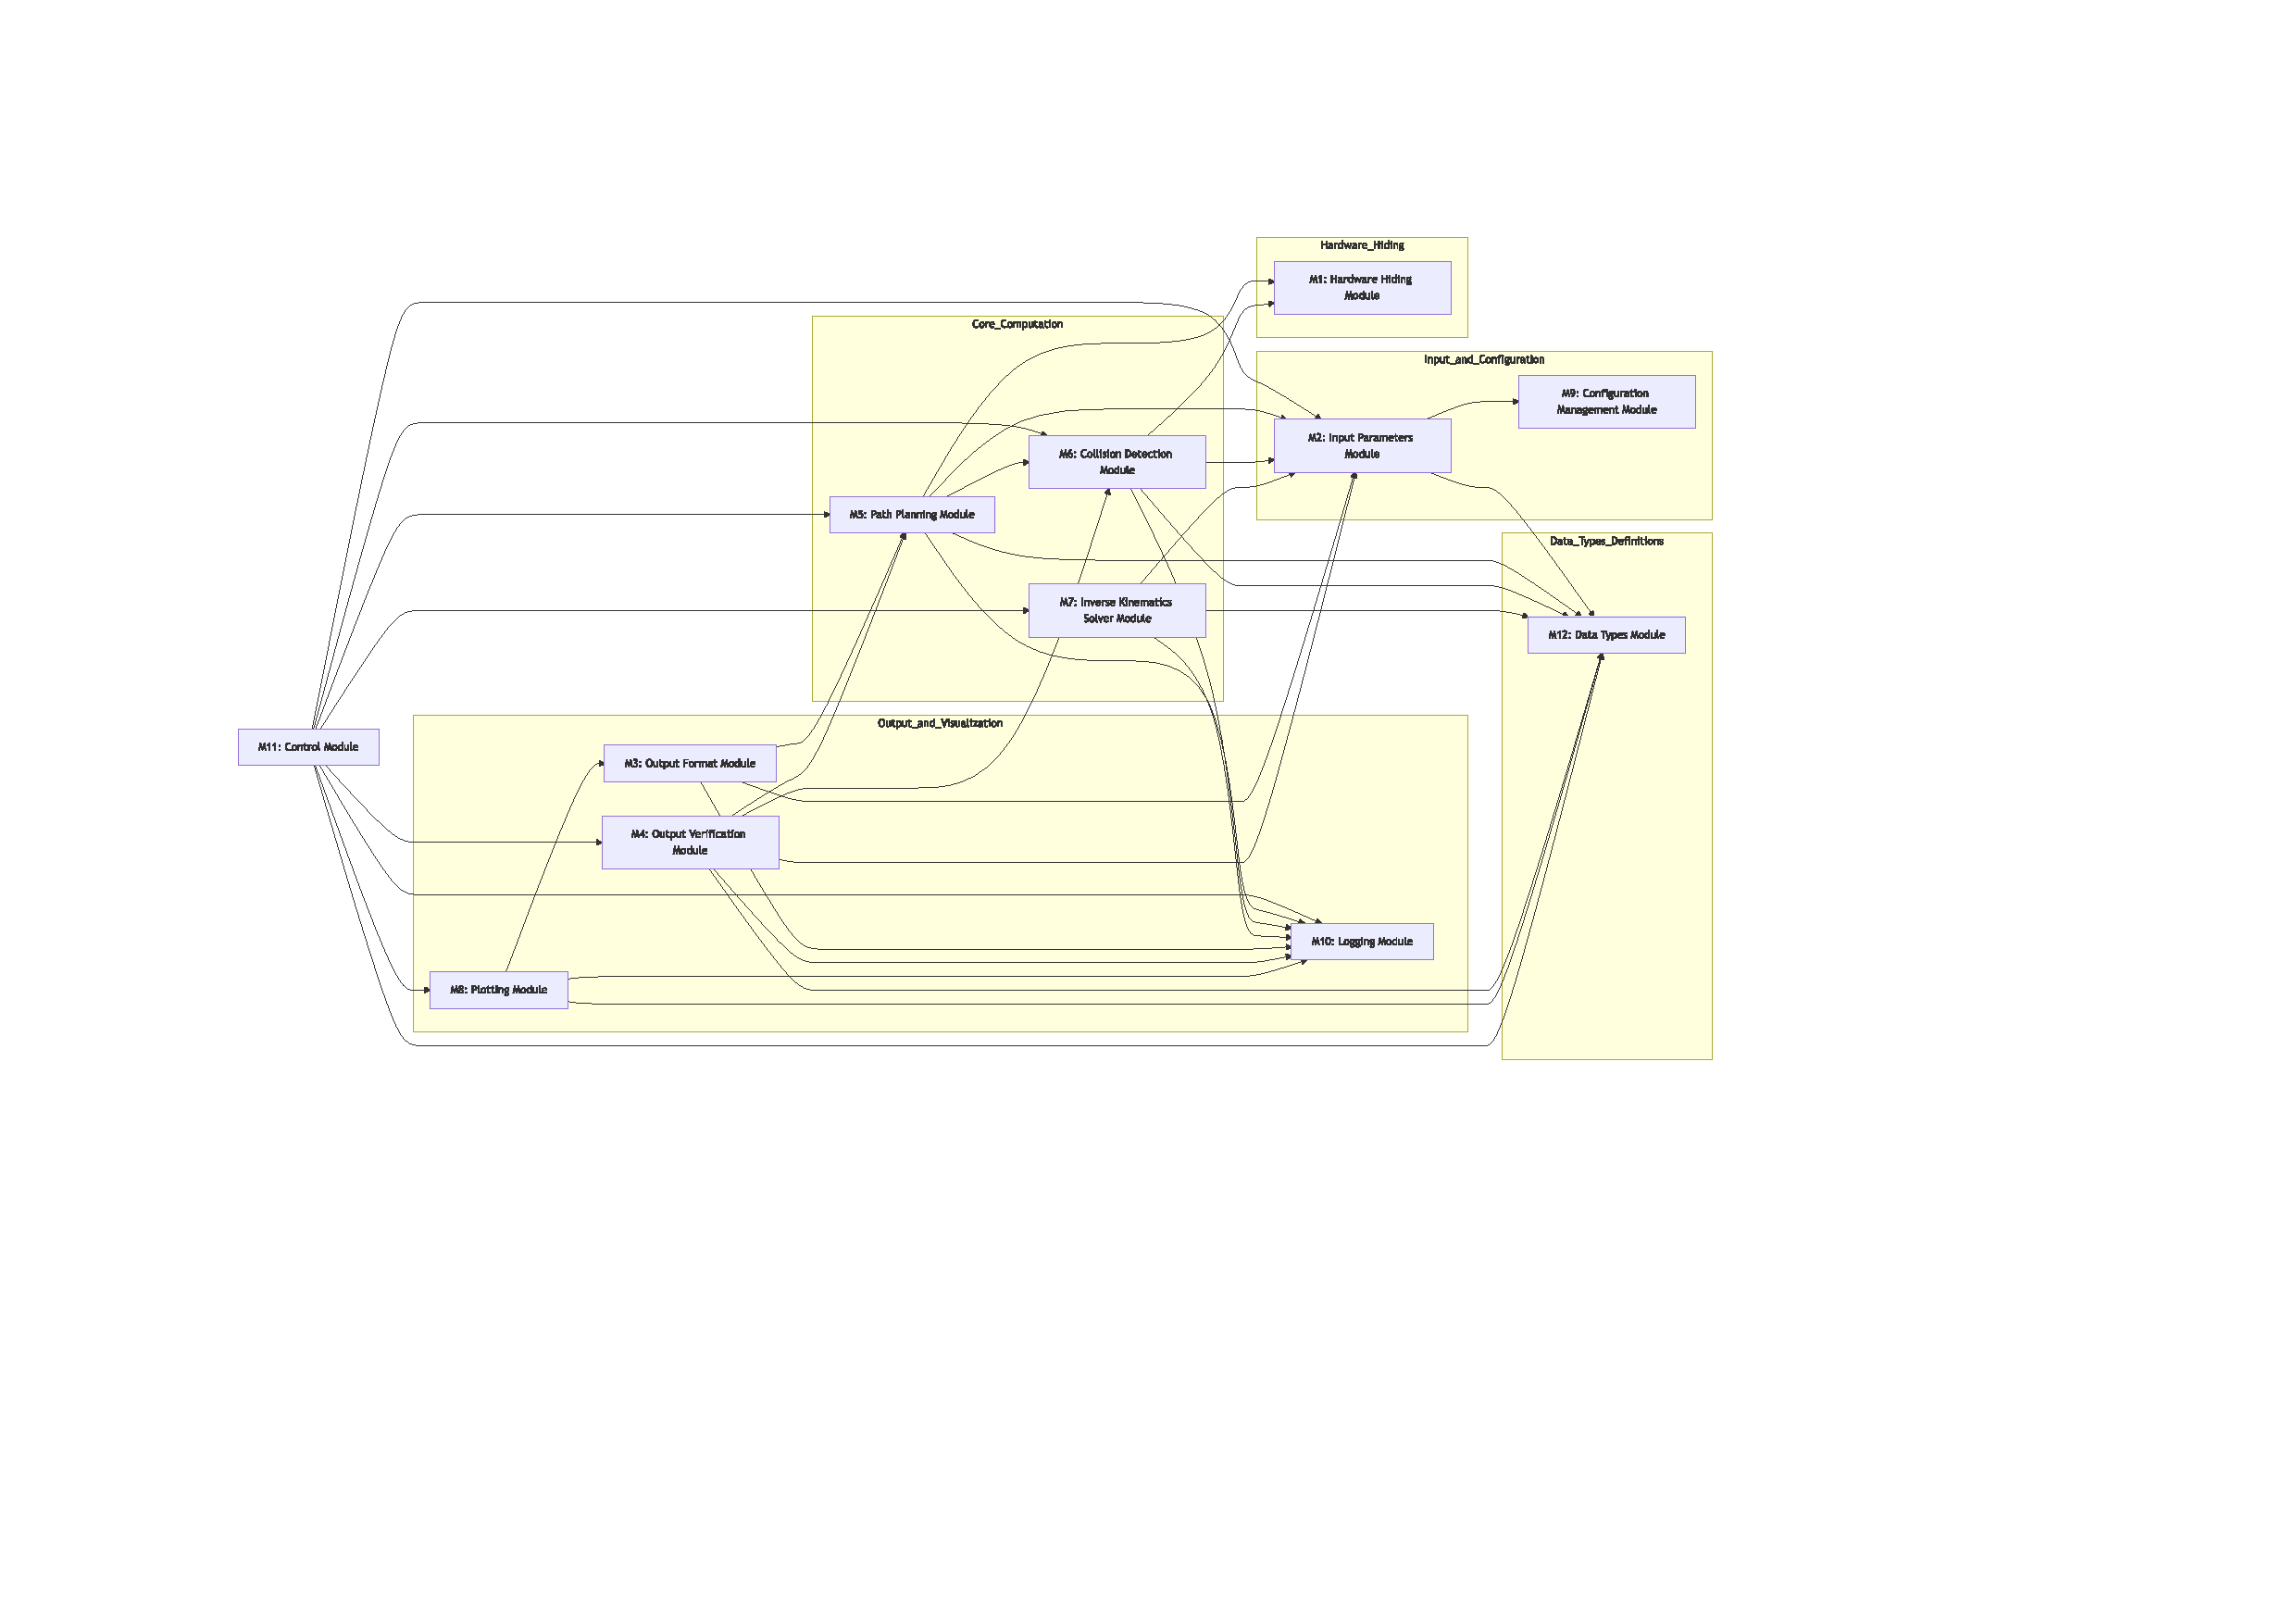
\includegraphics[width=1\textwidth]{figure2.pdf}
\caption{Use hierarchy among modules}
\label{FigUH}
\end{figure}

%\section*{References}

% \section{User Interfaces}

% \wss{Design of user interface for software and hardware.  Attach an appendix if
% needed. Drawings, Sketches, Figma}

\section{User Interface} \label{SecUI}

The user interface (UI) for the 2D robot arm path planning software is designed for ease of use, providing a clear workflow from data input to visualization of computed paths. Given the primary users are researchers, engineers, and developers, the interface emphasizes simplicity, clarity, and flexibility.

The main components of the user interface include:

\begin{itemize}
    \item \textbf{Input Configuration Panel:}  
    Allows users to define and modify input parameters such as robot arm lengths, initial and goal positions, obstacle coordinates, and other relevant constraints.

    \item \textbf{Visualization Window:}  
      Displays the robot arm configuration, obstacles, and computed collision-free paths clearly in a graphical manner. Users can visually inspect and verify planned paths interactively.

    \item \textbf{Control and Parameter Adjustment Panel:}  
      Provides interactive controls allowing users to adjust planning parameters, such as resolution of the planning grid, algorithm selection, and tolerances.

    \item \textbf{Logging and Debugging Output:}  
      Offers real-time logs and debugging information to facilitate tracing the planning process and to quickly identify any issues.

    \end{itemize}


% \section{Design of Communication Protocols}

% \wss{If appropriate}

% \section{Timeline}

% \wss{Schedule of tasks and who is responsible}

% \wss{You can point to GitHub if this information is included there}

\bibliographystyle {plainnat}
\bibliography{../../../refs/References}

\newpage{}

\end{document}